

\tikzset{every picture/.style={line width=0.75pt}} %set default line width to 0.75pt        

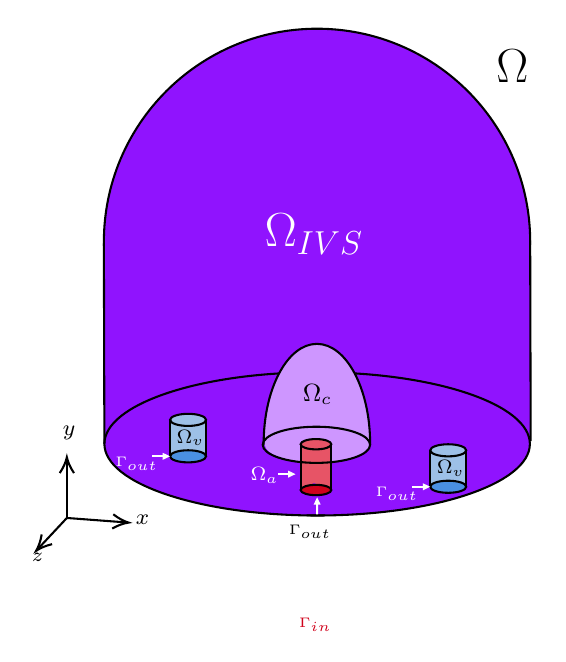
\begin{tikzpicture}[x=0.75pt,y=0.75pt,yscale=-1,xscale=1]
%uncomment if require: \path (0,300); %set diagram left start at 0, and has height of 300

%Shape: Polygon [id:ds01690740321670181] 
\draw  [draw opacity=0][fill={rgb, 255:red, 144; green, 19; blue, 254 }  ,fill opacity=1 ] (249.39,123.24) -- (249.64,219.89) -- (149,187.3) -- (44.25,221.25) -- (44,124.6) -- cycle ;
%Shape: Ellipse [id:dp07097539184655921] 
\draw  [fill={rgb, 255:red, 144; green, 19; blue, 254 }  ,fill opacity=1 ] (44.25,221.25) .. controls (44.25,202.2) and (90.14,186.75) .. (146.75,186.75) .. controls (203.36,186.75) and (249.25,202.2) .. (249.25,221.25) .. controls (249.25,240.3) and (203.36,255.75) .. (146.75,255.75) .. controls (90.14,255.75) and (44.25,240.3) .. (44.25,221.25) -- cycle ;
%Shape: Arc [id:dp2751562142003694] 
\draw  [draw opacity=0][fill={rgb, 255:red, 206; green, 150; blue, 255 }  ,fill opacity=1 ] (120.98,221.7) .. controls (120.98,221.54) and (120.98,221.37) .. (120.98,221.21) .. controls (120.98,194.62) and (132.46,173.06) .. (146.63,173.06) .. controls (160.79,173.06) and (172.28,194.62) .. (172.28,221.21) .. controls (172.28,221.37) and (172.28,221.53) .. (172.28,221.69) -- (146.63,221.21) -- cycle ; \draw   (120.98,221.7) .. controls (120.98,221.54) and (120.98,221.37) .. (120.98,221.21) .. controls (120.98,194.62) and (132.46,173.06) .. (146.63,173.06) .. controls (160.79,173.06) and (172.28,194.62) .. (172.28,221.21) .. controls (172.28,221.37) and (172.28,221.53) .. (172.28,221.69) ;  
%Shape: Polygon [id:ds05551048064302422] 
\draw  [draw opacity=0][fill={rgb, 255:red, 157; green, 192; blue, 231 }  ,fill opacity=1 ] (209.9,227.26) -- (218.57,224.34) -- (218.57,241.91) -- (209.9,238.99) -- (201.24,241.91) -- (201.24,224.34) -- cycle ;
%Straight Lines [id:da2434758497711771] 
\draw    (26.17,229.67) -- (26.17,256.94) ;
\draw [shift={(26.17,227.67)}, rotate = 90] [color={rgb, 255:red, 0; green, 0; blue, 0 }  ][line width=0.75]    (7.65,-3.43) .. controls (4.86,-1.61) and (2.31,-0.47) .. (0,0) .. controls (2.31,0.47) and (4.86,1.61) .. (7.65,3.43)   ;
%Straight Lines [id:da34708087552976474] 
\draw    (53.92,259.02) -- (26.17,256.94) ;
\draw [shift={(55.92,259.17)}, rotate = 184.27] [color={rgb, 255:red, 0; green, 0; blue, 0 }  ][line width=0.75]    (7.65,-3.43) .. controls (4.86,-1.61) and (2.31,-0.47) .. (0,0) .. controls (2.31,0.47) and (4.86,1.61) .. (7.65,3.43)   ;
%Straight Lines [id:da30935515392198853] 
\draw    (12.7,271.34) -- (26.17,256.94) ;
\draw [shift={(11.33,272.8)}, rotate = 313.09] [color={rgb, 255:red, 0; green, 0; blue, 0 }  ][line width=0.75]    (7.65,-3.43) .. controls (4.86,-1.61) and (2.31,-0.47) .. (0,0) .. controls (2.31,0.47) and (4.86,1.61) .. (7.65,3.43)   ;
%Shape: Arc [id:dp4353496030990409] 
\draw  [draw opacity=0][fill={rgb, 255:red, 144; green, 19; blue, 254 }  ,fill opacity=1 ] (44.01,125.8) .. controls (44,125.17) and (44,124.55) .. (44,123.92) .. controls (44,67.2) and (89.98,21.22) .. (146.7,21.22) .. controls (203.42,21.22) and (249.4,67.2) .. (249.4,123.92) .. controls (249.4,124.42) and (249.39,124.91) .. (249.39,125.41) -- (146.7,123.92) -- cycle ; \draw   (44.01,125.8) .. controls (44,125.17) and (44,124.55) .. (44,123.92) .. controls (44,67.2) and (89.98,21.22) .. (146.7,21.22) .. controls (203.42,21.22) and (249.4,67.2) .. (249.4,123.92) .. controls (249.4,124.42) and (249.39,124.91) .. (249.39,125.41) ;  
%Straight Lines [id:da13806152488339984] 
\draw    (44,124.6) -- (44.25,221.25) ;
%Straight Lines [id:da6383479755639994] 
\draw    (249.39,123.24) -- (249.64,219.89) ;
%Shape: Ellipse [id:dp9307891644906987] 
\draw  [fill={rgb, 255:red, 157; green, 192; blue, 231 }  ,fill opacity=1 ] (201.24,224.34) .. controls (201.24,222.73) and (205.12,221.43) .. (209.9,221.43) .. controls (214.69,221.43) and (218.57,222.73) .. (218.57,224.34) .. controls (218.57,225.95) and (214.69,227.26) .. (209.9,227.26) .. controls (205.12,227.26) and (201.24,225.95) .. (201.24,224.34) -- cycle ;
%Shape: Ellipse [id:dp9565465123212877] 
\draw  [fill={rgb, 255:red, 74; green, 144; blue, 226 }  ,fill opacity=1 ] (201.24,241.91) .. controls (201.24,240.29) and (205.12,238.99) .. (209.9,238.99) .. controls (214.69,238.99) and (218.57,240.29) .. (218.57,241.91) .. controls (218.57,243.52) and (214.69,244.82) .. (209.9,244.82) .. controls (205.12,244.82) and (201.24,243.52) .. (201.24,241.91) -- cycle ;
%Shape: Ellipse [id:dp9395551579921961] 
\draw  [draw opacity=0][fill={rgb, 255:red, 206; green, 150; blue, 255 }  ,fill opacity=1 ] (121.57,221.69) .. controls (121.57,216.98) and (132.92,213.16) .. (146.92,213.16) .. controls (160.93,213.16) and (172.28,216.98) .. (172.28,221.69) .. controls (172.28,226.4) and (160.93,230.23) .. (146.92,230.23) .. controls (132.92,230.23) and (121.57,226.4) .. (121.57,221.69) -- cycle ;
%Straight Lines [id:da37394575581946365] 
\draw    (218.57,224.34) -- (218.57,241.91) ;
%Straight Lines [id:da5923482443180503] 
\draw    (201.24,224.34) -- (201.24,241.91) ;
%Shape: Polygon [id:ds36655981362937773] 
\draw  [draw opacity=0][fill={rgb, 255:red, 231; green, 84; blue, 102 }  ,fill opacity=1 ] (146.19,223.89) -- (153.57,221.41) -- (153.57,243.47) -- (145.22,240.09) -- (138.8,243.47) -- (138.8,221.41) -- cycle ;
%Straight Lines [id:da12421975552257325] 
\draw    (138.8,221.41) -- (138.8,243.47) ;
%Straight Lines [id:da06433371565445012] 
\draw    (153.57,221.41) -- (153.57,243.47) ;
%Shape: Ellipse [id:dp9306496239950879] 
\draw  [fill={rgb, 255:red, 231; green, 84; blue, 102 }  ,fill opacity=1 ] (138.8,221.41) .. controls (138.8,220.04) and (142.11,218.92) .. (146.19,218.92) .. controls (150.26,218.92) and (153.57,220.04) .. (153.57,221.41) .. controls (153.57,222.78) and (150.26,223.89) .. (146.19,223.89) .. controls (142.11,223.89) and (138.8,222.78) .. (138.8,221.41) -- cycle ;
%Straight Lines [id:da9919027107135354] 
\draw [color={rgb, 255:red, 255; green, 255; blue, 255 }  ,draw opacity=1 ]   (133.33,235.83) -- (127.67,235.83) ;
\draw [shift={(136.33,235.83)}, rotate = 180] [fill={rgb, 255:red, 255; green, 255; blue, 255 }  ,fill opacity=1 ][line width=0.08]  [draw opacity=0] (3.57,-1.72) -- (0,0) -- (3.57,1.72) -- cycle    ;
%Shape: Ellipse [id:dp6340587055082747] 
\draw   (120.53,221.69) .. controls (120.53,216.88) and (132.11,212.98) .. (146.4,212.98) .. controls (160.69,212.98) and (172.28,216.88) .. (172.28,221.69) .. controls (172.28,226.5) and (160.69,230.4) .. (146.4,230.4) .. controls (132.11,230.4) and (120.53,226.5) .. (120.53,221.69) -- cycle ;
%Straight Lines [id:da4747494457620296] 
\draw [color={rgb, 255:red, 255; green, 255; blue, 255 }  ,draw opacity=1 ]   (198.24,241.91) -- (192.57,241.91) ;
\draw [shift={(201.24,241.91)}, rotate = 180] [fill={rgb, 255:red, 255; green, 255; blue, 255 }  ,fill opacity=1 ][line width=0.08]  [draw opacity=0] (3.57,-1.72) -- (0,0) -- (3.57,1.72) -- cycle    ;
%Shape: Polygon [id:ds6448294514764339] 
\draw  [draw opacity=0][fill={rgb, 255:red, 157; green, 192; blue, 231 }  ,fill opacity=1 ] (84.57,212.59) -- (93.24,209.68) -- (93.24,227.24) -- (84.57,224.32) -- (75.9,227.24) -- (75.9,209.68) -- cycle ;
%Shape: Ellipse [id:dp5042958695035071] 
\draw  [fill={rgb, 255:red, 157; green, 192; blue, 231 }  ,fill opacity=1 ] (75.9,209.68) .. controls (75.9,208.07) and (79.78,206.76) .. (84.57,206.76) .. controls (89.36,206.76) and (93.24,208.07) .. (93.24,209.68) .. controls (93.24,211.29) and (89.36,212.59) .. (84.57,212.59) .. controls (79.78,212.59) and (75.9,211.29) .. (75.9,209.68) -- cycle ;
%Shape: Ellipse [id:dp621045676508921] 
\draw  [fill={rgb, 255:red, 74; green, 144; blue, 226 }  ,fill opacity=1 ] (75.9,227.24) .. controls (75.9,225.63) and (79.78,224.32) .. (84.57,224.32) .. controls (89.36,224.32) and (93.24,225.63) .. (93.24,227.24) .. controls (93.24,228.85) and (89.36,230.16) .. (84.57,230.16) .. controls (79.78,230.16) and (75.9,228.85) .. (75.9,227.24) -- cycle ;
%Straight Lines [id:da6241652370301061] 
\draw    (93.24,209.68) -- (93.24,227.24) ;
%Straight Lines [id:da7595036939515529] 
\draw    (75.9,209.68) -- (75.9,227.24) ;
%Straight Lines [id:da6580144119581173] 
\draw [color={rgb, 255:red, 255; green, 255; blue, 255 }  ,draw opacity=1 ]   (72.9,227.24) -- (67.24,227.24) ;
\draw [shift={(75.9,227.24)}, rotate = 180] [fill={rgb, 255:red, 255; green, 255; blue, 255 }  ,fill opacity=1 ][line width=0.08]  [draw opacity=0] (3.57,-1.72) -- (0,0) -- (3.57,1.72) -- cycle    ;
%Straight Lines [id:da516421428956964] 
\draw [color={rgb, 255:red, 255; green, 255; blue, 255 }  ,draw opacity=1 ]   (146.76,249.98) -- (146.75,255.75) ;
\draw [shift={(146.76,246.98)}, rotate = 90.08] [fill={rgb, 255:red, 255; green, 255; blue, 255 }  ,fill opacity=1 ][line width=0.08]  [draw opacity=0] (3.57,-1.72) -- (0,0) -- (3.57,1.72) -- cycle    ;
%Shape: Arc [id:dp001845141988116028] 
\draw  [draw opacity=0] (150.65,255.68) .. controls (149.31,255.7) and (147.97,255.71) .. (146.63,255.71) .. controls (144.98,255.71) and (143.34,255.7) .. (141.7,255.67) -- (146.63,221.21) -- cycle ; \draw   (150.65,255.68) .. controls (149.31,255.7) and (147.97,255.71) .. (146.63,255.71) .. controls (144.98,255.71) and (143.34,255.7) .. (141.7,255.67) ;  
%Shape: Ellipse [id:dp7362360871362295] 
\draw  [fill={rgb, 255:red, 208; green, 2; blue, 27 }  ,fill opacity=1 ] (138.8,243.47) .. controls (138.8,242.1) and (142.11,240.98) .. (146.19,240.98) .. controls (150.26,240.98) and (153.57,242.1) .. (153.57,243.47) .. controls (153.57,244.84) and (150.26,245.95) .. (146.19,245.95) .. controls (142.11,245.95) and (138.8,244.84) .. (138.8,243.47) -- cycle ;

% Text Node
\draw (27.27,221.01) node [anchor=south] [inner sep=0.75pt]  [font=\footnotesize]  {$y$};
% Text Node
\draw (57.88,257.72) node [anchor=west] [inner sep=0.75pt]  [font=\footnotesize]  {$x$};
% Text Node
\draw (7.79,276.08) node [anchor=west] [inner sep=0.75pt]  [font=\scriptsize]  {$z$};
% Text Node
\draw (145.32,120.23) node  [font=\LARGE,color={rgb, 255:red, 255; green, 255; blue, 255 }  ,opacity=1 ]  {$\Omega _{\text{IVS}}$};
% Text Node
\draw (146.92,197.43) node  [font=\small,color={rgb, 255:red, 0; green, 0; blue, 0 }  ,opacity=1 ]  {$\Omega _{\text{c}}$};
% Text Node
\draw (129.63,236.34) node [anchor=east] [inner sep=0.75pt]  [font=\scriptsize,color={rgb, 255:red, 255; green, 255; blue, 255 }  ,opacity=1 ]  {$\Omega _{\text{a}}$};
% Text Node
\draw (211.09,233.02) node  [font=\scriptsize,color={rgb, 255:red, 0; green, 0; blue, 0 }  ,opacity=1 ]  {$\Omega _{\text{v}}$};
% Text Node
\draw (240.82,39.23) node  [font=\LARGE,color={rgb, 255:red, 0; green, 0; blue, 0 }  ,opacity=1 ]  {$\Omega $};
% Text Node
\draw (145.93,303.53) node [anchor=north] [inner sep=0.75pt]  [font=\tiny,color={rgb, 255:red, 208; green, 2; blue, 27 }  ,opacity=1 ]  {$\Gamma _{\text{in}}$};
% Text Node
\draw (196.83,240.77) node [anchor=north east] [inner sep=0.75pt]  [font=\tiny,color={rgb, 255:red, 255; green, 255; blue, 255 }  ,opacity=1 ]  {$\Gamma _{\text{out}}$};
% Text Node
\draw (85.75,218.35) node  [font=\scriptsize,color={rgb, 255:red, 0; green, 0; blue, 0 }  ,opacity=1 ]  {$\Omega _{\text{v}}$};
% Text Node
\draw (71.5,226.1) node [anchor=north east] [inner sep=0.75pt]  [font=\tiny,color={rgb, 255:red, 255; green, 255; blue, 255 }  ,opacity=1 ]  {$\Gamma _{\text{out}}$};
% Text Node
\draw (155,268.36) node [anchor=south east] [inner sep=0.75pt]  [font=\tiny,color={rgb, 255:red, 0; green, 0; blue, 0 }  ,opacity=1 ]  {$\Gamma _{\text{out}}$};


\end{tikzpicture}
